\chapter{Referencial Teórico}
\label{ch:referencial}
\hspace{2.5cm}

Este capítulo objetiva a apresentar os principais conceitos que serão utilizados na metodologia. Tais conceitos são referentes ao desenvolvimento web e serão cruciais para o entendimento do trabalho essencialmente porque tais informações servirão de bases fundamentais para o disposto no Capítulo \ref{ch:metodologia}.

Na Seção \ref{sec:engenhariaweb} será revisado o significado de Engenharia Web e sua importância. Na Seção \ref{sec:metodologiaagil} o conteúdo terá enfoque nas metodologias ágeis, ocorrendo, posteriormente, uma breve comparação entre as mais conhecidas. A Seção \ref{sec:cms}, por sua vez, irá explanar sobre a utilização de Sistemas de Gerenciamento ou Gestão de Conteúdo na construção de aplicações na internet. A Seção \ref{sec:vps} fará uma sucinto resumo sobre os Servidores Virtuais Privados e os benefícios do seu emprego. Os conceitos referentes às ferramentas e tecnologias empregadas entre os materiais e métodos do trabalho serão brevemente tratados na Seção \ref{sec:ferramentas}, a fim de proporcionar ao leitor uma compreensão antecipada sobre tais assuntos. Por fim, a Seção \ref{sec:trabalhoscorrelatos} revelará alguns trabalhos desenvolvidos com enfoque na implementação de sites e/ou sistemas organizacionais. 

\hspace{2.5cm}

\section{Engenharia Web}
\label{sec:engenhariaweb}
%Seção: Engenharia Web 
\hspace{2.5cm}

\citeonline{ginige2001web} classificam a Engenharia Web como um conjunto de técnicas que propõe o estabelecimento de informações científicas para desenvolver princípios e abordagens disciplinadas para a conquista do sucesso no desenvolvimento de sistemas web. 

Para facilitar o entendimento, pode-se concluir que a Engenharia Web se caracteriza pela estipulação de métodos e procedimentos que podem ser adotados por toda a equipe para auxiliar no desenvolvimento do projeto de aplicações web.

As metodologias de desenvolvimento de software, estudadas em subáreas da engenharia de software, podem ser adotadas para organizar todo o projeto de desenvolvimento de um software. Elas podem ser divididas entre tradicionais e ágeis, e são operadas para auxiliar na produção de software em processos como a análise de requisitos e a codificação, como mencionado por \citeonline{dos2004comparaccao}. \apudonline[~p. 1]{Sommerville}{dos2004comparaccao} define quatro atividades comuns a todos os processos de desenvolvimento:

\begin{itemize}
 \item \textbf{Especificação de Software}: etapa em que ocorre um contato maior da equipe com os clientes, com o intuito de determinar os requisitos e funcionalidades do programa. Para tal, existem diversas formas de coletar essas informações, como por exemplo realização de entrevistas, questionários, observação naturalista, entre outras;
 \item \textbf{Projeto e Implementação de Software}: etapa de construção de diagramas para gerar modelos que serão posteriormente implementados;
 \item \textbf{Validação de Software}: é a fase de verificação dos requisitos. Nesta etapa acontece uma análise de requisitos atendidos e não atendidos; e
 \item \textbf{Evolução do Software}: diferentemente das demais, esta fase é posterior à entrega do produto ao cliente. Ela corresponde basicamente às manutenções e atualizações de software que serão produzidas com o passar do tempo para que ele possa continuar sendo utilizado pelos usuários.
\end{itemize}

\hspace{2.5cm}

\section{Metodologias Ágeis}
\label{sec:metodologiaagil}
%metodologia ágil
\hspace{2.5cm}

Os métodos ágeis surgiram na década de 90 para alterar a mentalidade das equipes de desenvolvimento da época, contradizendo os métodos tradicionais eliminando gasto com documentação excessiva, enfatizando a comunicação e aumentandoí a proximidade com o cliente para produzir software de qualidade \cite{sato2007uso}.

Segundo \citeonline{conforto2009gerenciamento}, a assinatura do manifesto ágil \footnote{Disponível em: \textsf{http://agilemanifesto.org/}} foi um marco para o nascimento das metodologias ágeis. O manifesto se trata de um documento em que a eficácia das metodologias tradicionais é questionada em cenários que envolvam incertezas e constantes mudanças no ambiente empresarial. 

É importante ressaltar que tais metodologias podem ser aplicadas tanto em equipes menores, de desenvolvimento, por exemplo, quanto em projetos inteiros através do Gerenciamento Ágil de Projetos (GAP), constituídos por várias equipes. Também é interessante saber que um dos fundamentos do processo ágil é a construção de ciclos, cujo objetivo é adaptar e avaliar constantemente o produto antes que chegue no estado final, objetivando atribuí-lo qualidade perante os requisitos estipulados e a satisfação do cliente.

A seguir, estão descritos alguns dos principais métodos de desenvolvimento de software existentes. Para o primeiro deles, \textit{Scrum}, foram descritos mais detalhes em relação aos demais por dois motivos principais: além de ser uma das metodologias, ou \textit{framework}, mais conhecidas e utilizadas atualmente, como demonstra a Figura \ref{ageis-microsoft}, ela também possui aspectos em comum com outras, tais como conceitos referentes a coleta de requisitos, retrospectivas, reuniões em pé e duração das \textit{sprints}, podendo esta ser nomeada como ciclos, o que varia de método para método.


\textbf{\textit{Scrum}}: O \textit{Scrum} é um processo para construção incremental de softwares em ambientes complexos e provê o desenvolvimento de softwares em curtas iterações, denominadas \textit{sprints} \cite{rising2000scrum}.

\textit{Sprints}: cada \textit{sprint} inclui todas as fases de um software modelo de ciclo de vida de desenvolvimento, como design, implementação, testes, revisão de clientes, etc \cite[~p. 2, tradução nossa]{matharu2015empirical}. Elas têm duração de até 30 dias e também compreendem o procedimento de adaptação a mudança de variáveis (requisitos, tempo, recursos, tecnologia), pois em seu término há sempre uma reflexão sobre as tarefas, definidas antes do início do ciclo, que foram realizadas com sucesso e os próximos incrementos ou revisões as serem executados nas próximas \textit{sprints}, de acordo com o \textit{feedback} passado na reunião com o cliente \citeonline{awad2005comparison}. 

Existem cinco características únicas para o desenvolvimento baseado em \textit{Scrum} \cite{matharu2015empirical}, são eles:

\begin{enumerate}
 \item Colaboração: a promoção da colaboração se dá pelo fato do desenvolvimento ser conduzido por equipes compostas por pessoas multifuncionais, envolvendo programadores, arquitetos de software e especialistas em qualidade de software.
 
 \item Encontros diários: são reuniões de curta duração, comandadas pelo \textit{Scrum Master}, onde as equipes de desenvolvimento se comunicam e discutem o progresso com que os requisitos encontrados no \textit{product backlog} estão sendo implementados \cite{rising2000scrum} afirma que esses encontros podem ser realizados três ou quatro vezes na semana e neles os assuntos mais frequentes se baseiam nas dificuldades encontradas e como vencer os obstáculos até a próxima reunião.
 
 \item \textit{Product Backlog}: o \textit{product backlog} captura os requisitos que devem ser implementados, sendo ordenados por nível prioridade. Ele ainda contém erros resolvidos, características gerais e requisitos não funcionais do software.
 
 \item \textit{Sprint Backlog}: este item registra a lista de tarefas que deverão ser realizadas durante a próxima \textit{sprint}. Logicamente a lista de tarefas deve ser baseada no rendimento das equipes para que não haja um planejamento de quantidade de itens exorbitante que dificilmente serão cumpridos. 
 
 \item Regras: são regras fundamentais da metodologia segundo \citeonline{matharu2015empirical}:
 \begin{itemize}
  \item PO \textit{(Product Owner)}: ``responsável pela definição, priorização e comunicação dos requisitos de produto e guias do processo de desenvolvimento'' \cite[~p. 3, tradução nossa]{matharu2015empirical}.
  
  \item Time de desenvolvimento: equipes compostas de 3 a 9 indivíduos responsáveis por executar as tarefas previstas pelo PO.
 
  \item \textit{Scrum Master}: responsável por guiar as equipes no respeito às regras e princípios do \textit{Scrum}. Ele remove impedimentos e auxilia no processo de desenvolvimento.
  
 \end{itemize}
 
\end{enumerate}


Em pesquisa realizada pelo \textit{State of Agile Report} (Estado de Relatório Rápido, em português), em 2019, 72\% das empresas que participaram responderam praticar com \textit{Scrum} ou uma metodologia híbrida que o utiliza como metodologia de desenvolvimento. Tal pesquisa, encontrada em \citeonline{relatorioAnual2019}, foi realizada pela décima terceira vez em 2019 e coletou informações sobre metodologias de processos e desenvolvimento de empresas e organizações da Europa, Ásia, América do Sul e África dos mais variados ramos, tais como de tecnologia, de transporte, industrial, governamental e energético.

Os resultados obtidos com a pesquisa identificam a importância de se conhecer a metodologia estudada nesta seção e como ela ainda é usada por empresas do mundo inteiro. Com o objetivo de assegurar e dar ainda mais veracidade a esta conclusão, outra pesquisa, esta realizada em funcionários da empresa de tecnologia \textit{Microsoft} e via web, detalhada em \citeonline{begel2007usage}, aponta que, das 192 respostas recebidas, a maioria das pessoas que trabalham com desenvolvimento, testes e funções de gerenciamento diretamente ligadas a produção de software aplicam o \textit{Scrum} como a metodologia padrão para construir seus produtos, como representado na Figura \ref{ageis-microsoft}. 

\begin{figure}[htb]
 \centering
 \caption{Diferentes metodologias utilizadas pelos funcionários}
 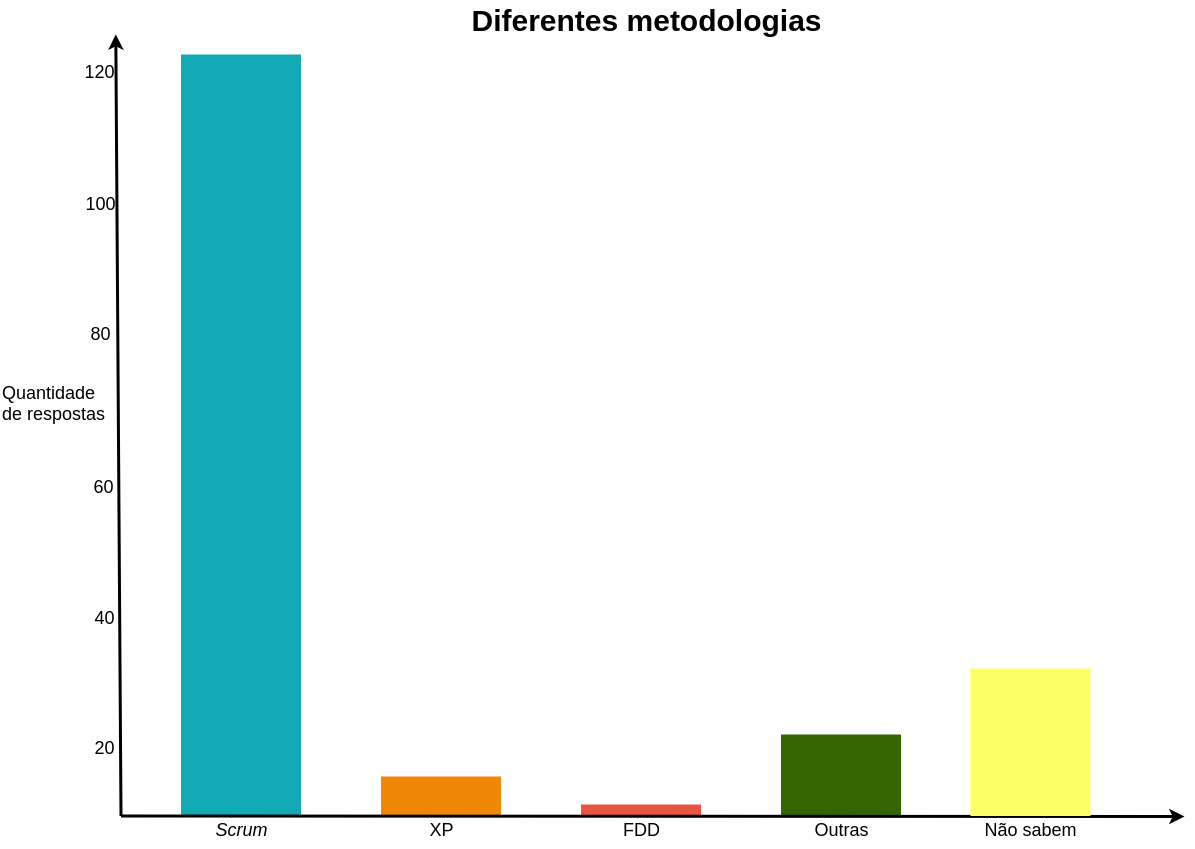
\includegraphics[width=0.8\textwidth]{figuras/diferentes-metodologias}
 \fonte{\citeonline{begel2007usage}. Adaptado.}
 \label{ageis-microsoft}
\end{figure}

Ainda sobre o \textit{Scrum}, \citeonline{PAHUJA2015} informa que há a possibilidade de se utilizá-lo de maneira individual, e ainda destaca quatro características importantes para aplicá-lo nesse cenário, são elas: faça o que você pode com o que você tem, tenha constante auto reflexão, trabalhe com objetivos curtos e bem definidos e planeje todo o trabalho sobre \textit{sprints}.

A título de conhecimento sobre demais métodos ágeis, o artigo de \citeonline{sato2007uso} emerge sobre os seguintes métodos:


\textbf{\textit{Extreme Programming} (XP)}: juntamente com o \textit{Scrum} é o mais utilizado. Busca ``a excelência no desenvolvimento de software, visando baixo custo, poucos defeitos, alta produtividade e alto retorno de investimento'' \cite{sato2007uso}.


\textbf{\textit{Lean Software Development}}: baseado no sistema de produção da Toyota, este método revolucionou a manufatura, o desenvolvimento de produtos e o gerenciamento da cadeia de suprimentos. Sustentado sobre sete princípios: ``Elimine Desperdícios'', ``Inclua a Qualidade no Processo'', ``Crie Conhecimento'', ``Adie comprometimentos'', ``Entregue rápido'', ``Respeite as pessoas'' e ``Otimize o Todo'' \cite{sato2007uso};
 
 
\textbf{Metodologia da família \textit{Crystal}}: possui uma peculiaridade, a ``habitabilidade'', que significa ``o mínimo de processo necessário para que a equipe consiga ter sucesso'' \cite{sato2007uso}. Além disso, seus métodos compartilham propriedades como: entrega frequente, reflexão e comunicação;


\textbf{\textit{Feature Driven Development} (FDD)}: criada na década de 90, ele se aproveita de diagramas UML para representar classes de diferentes responsabilidades e é constituído por duas fases: a de concepção e planejamento e a iterativa de construção, compostas por 5 processos internos ao todo;


\textbf{\textit{Adaptive Software Development}}: método que propõe três fases possivelmente sobrepostas: especulação, colaboração e aprendizado. Aqui, o conhecimento sobre falhas, oriundas de falsas premissas, é adquirido por meio de curtas iterações, sendo corrigidas vagarosamente;


\textbf{\textit{Dynamic systems development method} (DSDM)}: seu desenvolvimento se iniciou em 1994 e possui duas fases primárias, uma de viabilidade, cujo objetivo é verificar se é viável a execução deste método na situação decorrente, e um estudo de negócio para definir os requisitos iniciais e a arquitetura de software. No decorrer do processo ainda são previstas etapas para prototipação, construção do sistema e entrega do produto. O DSDM ainda possui princípios básicos relacionados à frequência de entregas e de testes, e participação direta do usuário durante todo o processo; e


Concluindo o tema, é aconselhável exibir as diferenças entre os dois tipos de metodologias, para isso o Quadro \ref{comparativo-metodologias} foi criado.

\begin{quadro}[h]
\centering
\scalefont{0.7}
\caption{Diferenças básicas entre metodologias tradicionais e metodologias ágeis}
\vspace{0.5cm}

\setlength{\extrarowheight}{0.25cm}
\begin{tabular}{|L|L|L|}
\hline
\textbf{Características} & \textbf{Gerenciamento Tradicional} & \textbf{Gerenciamento Ágil} \\ % Note a separação de col. e a quebra de linhas
\hline
Ter definido a priori & Escopo & Tempo (\textit{sprints})\\
\hline
Responsável pela organização para \ atingir os objetivos do projeto & Gerente de projeto & \textit{Scrum master}\\
\hline
Frequência de reuniões de status & Dependendo da complexidade/necessidade do projeto & Diárias\\
\hline
Escopo & Bem definido nas fases iniciais do projeto & Definido em alto nível e os requisitos definidos de forma iterativa\\
\hline
Tempo & Cronograma detalhado para realização de todo o projeto & Cronograma orientado a produto com entregas incrementais\\
\hline
Custo & Monitoração das alterações para que não altere o custo planejado & Maior controle em função da rapidez em alterações\\
\hline
Qualidade & Processo de verificação, validação e plano de testes & Programação em pares, testes incrementais e refatoração\\
\hline
Riscos & Análise de riscos durante todo o ciclo de vida do projeto & Aplica-se o mesmo conceito do gerenciamento tradicional\\
\hline
Comunicação & Documentação e formal & Implícita, interpessoal e colaborativa\\

\hline
\end{tabular}
\fonte{\citeonline{dos2013metodologias}. Adaptado.}
\label{comparativo-metodologias}
\end{quadro}


Através de uma observação do Quadro \ref{comparativo-metodologias} é possível notar diferenças primordiais entre o gerenciamento tradicional e o ágil. Dentre as informações apresentadas, destacam-se a forma de comunicação, a frequência de reuniões de status e o elemento a ser definido prioritariamente, porque são características totalmente diferentes entre as duas metodologias independentemente das customizações que possam ser feitas para determinados projetos. 

Segundo conteúdo publicado no diário \citeonline{dingsoyr2012decade} as duas metodologias ágeis mais comuns em equipes de desenvolvimento de software são o \textit{Extreme Programming} e o \textit{Scrum}, ambas estão diferenciadas na Tabela \ref{scrumVSxp}.

\begin{table}[h]
\centering
\scalefont{0.7}
\caption{Comparação entre o XP e o \textit{Scrum}}
\vspace{0.5cm}

\setlength{\extrarowheight}{0.25cm}
\begin{tabular}{L|L|L}
 
\textbf{Recursos} & \textbf{\textit{Extreme Programming}} & \textbf{\textit{Scrum}}  \\ % Note a separação de col. e a quebra de linhas
\hline                               % para uma linha horizontal
Tamanho do projeto & Pequeno & Todos \\
Tamanho das equipes (pessoas) & 2 a 10 & Menores que 10 \\
Duração das \textit{sprints} (semanas) & 1 a 3 & 4 \\
Elicitação de requisitos & Histórias de usuário & Não definido \\
Mudanças durante a iteração & Permitido & Não permitido \\          % não é preciso quebrar a última linha
Ordem de desenvolvimento definida por & Cliente & Equipe \textit{Scrum} \\
Envolvimento do \textit{stakeholder} & Durante o processo & Não definido \\
\hline
\end{tabular}
\fonte{\citeonline{anwer2017comparative}. Adaptado.}
\label{scrumVSxp}
\end{table}


\hspace{2.5cm}
\section{Sistemas de Gerenciamento de Conteúdo}
\label{sec:cms}
%CMS
\hspace{2.5cm}

O \textit{Content Management System} (CMS), ou Sistema de Gerenciamento de Conteúdo (SGC), em português, surgiu, segundo \citeonline{chagas2018estudo},
no final da década de 90 com o intuito de melhorar a gestão do conteúdo dos \textit{websites} das organizações da época.  

\citeonline{meike2009security} e \citeonline{chagas2018estudo} citam qualidades proporcionadas aos desenvolvedores que os utilizam.
Segundo eles as organizações podem utilizar um sistema de gerenciamento de conteúdo para construir \textit{websites},
lojas on-line ou portais, havendo redução de erros de publicação que facilitam o processo de validação e sendo manuseados por muitas
pessoas sem que seja necessário editar o código-fonte e possuir conhecimento especializado na área de programação.

Outro fator positivo encontrado nesses sistemas é a possibilidade de colaboração entre os desenvolvedores. Porque uma aplicação web desenvolvida em um CMS pode ser gerenciada por diversas pessoas, podendo ter restrições de acesso de cada uma delas a diferentes partes do sistema, ou seja, é possível definir níveis de acesso a usuários para que cada um deles possa administrar um ou mais tipos de conteúdo do mesmo. Para sintetizar, \apud[~p. 1]{boiko}{chagas2018estudo} conclui que ``um SGC possibilita a criação, o gerenciamento, a distribuição, a publicação e a recuperação de informações corporativas''.

Esses sistemas possuem características próprias que variam de acordo com o tipo de sistema. Existem CMSs baseados nas linguagens de programação Python, Java, PHP e Perl, sendo aspectos disjuntos aos sistemas, porém todos eles são capazes de usar linguagens padrão da web e bancos de dados relacionais, como visto na Figura \ref{figura3}.

\begin{figure}[htb]
 \centering
 \caption{Sistemas de Gerenciamento de Conteúdo da web de código aberto e tecnologias relacionadas}
 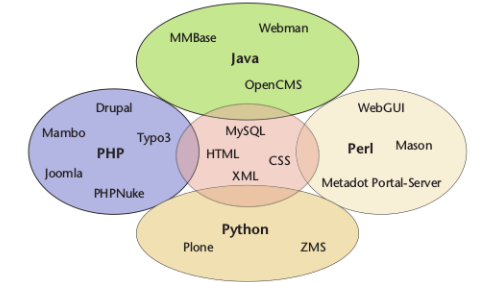
\includegraphics[width=0.7\textwidth]{figuras/linguagens-cms-1}
 \fonte{\citeonline{meike2009security}.}
 \label{figura3}
\end{figure}

\newpage
As próximas subseções foram dedicadas a gerar uma maior compreensão sobre os Sistemas de Gerenciamento de Conteúdo e sua utilização em âmbito institucional. Através delas será possível assimilar os diferentes tipos de sistemas de gestão e seus principais atributos, estabelecendo ainda um comparativo entre eles no que diz respeito à suas características e utilização em meio corporativo.

\hspace{2.5cm}

\subsection{Tipos de Sistemas de Gerenciamento de Conteúdo}
\label{subsec:tipos-cms}
\hspace{2.5cm}

É possível encontrar centenas de ferramentas de gerenciamento de conteúdo hoje em dia, sendo que, as questões que os diferem são diversas, citando-se requisitos do sistema, segurança, suporte, facilidade de uso e desempenho \cite{dasoluccao}.

No relatório \textit{Open Source CMS Market Share Report} divulgado pela agência digital \citeonline{relatoriocms}, foi possível obter a correlação entre os diferentes CMSs com os principais sites encontrados no \textit{Google PageRank}. O \textit{Google PageRank} é ``um método usado pela Google para determinar a importância ou a relevância de uma página. Páginas relevantes têm altos escalões e provavelmente aparecerão no topo nos resultados de pesquisa'' \cite[~p. 3, tradução nossa]{mirdha2014comparative}. A correlação está disponível na Tabela \ref{pagerank}.


\begin{table}[h]
\centering
\scalefont{0.7}
\caption{Ranking das páginas por CMS}
\vspace{0.5cm}

\setlength{\extrarowheight}{0.15cm}
\begin{tabular}{L|L}
 
\textbf{\textit{Content Management System}} & \textbf{\textit{Page Rank}} \\ % Note a separação de col. e a quebra de linhas
\hline                               % para uma linha horizontal
\textit{Joomla!} & 9 \\
\textit{Drupal}  & 9 \\
\textit{WordPress} & 9 \\
\textit{Plone} & 9 \\
\textit{Typo3} & 8  \\          % não é preciso quebrar a última linha
\textit{Concrete5} & 7 \\
\textit{DotNetNuke} & 7 \\
\textit{Alfresco} & 7 \\
\hline
\end{tabular}
\fonte{\apudonline{relatoriocms}{mirdha2014comparative}. Adaptado.}
\label{pagerank}
\end{table}

\newpage

A relevância das páginas é proporcional ao ranking e indica que quanto maior ele seja, mais chance a página tem de aparecer
no topo da lista dos resultados de uma pesquisa do mecanismo de busca da Google.

Por conveniência, os quatro sistemas mais bem colocados serão os escolhidos para dar início ao processo de comparação entre os principais. Tal processo se encontra na Subseção \ref{subsec:comparacao}, desenvolvida adiante. Porém, antes de iniciá-la, é importante haver uma apresentação dos sistemas escolhidos para deixar claro as distinções básicas entre eles antes de adentrar em seus detalhes e especificidades.

\textbf{\textit{Drupal}}: o CMS é derivado de um projeto escrito por um universitário holandês que tinha como objetivo fornecer meios de compartilhar notícias e eventos \cite{menezes2016processo}. Seu projeto foi considerado \textit{open source} (código aberto) em 2001 e baseou-se na linguagem de programação PHP. Para empregá-lo é necessário possui uma máquina que suporte um servidor web do PHP com versão de 5.2 ou superior, exemplos: \textit{Apache, nginx} e \textit{IIS}, além de um banco de dados, exemplos: MySQL, \textit{SQLite} e \textit{PostgreSQL} \cite{tomlinson2010beginning}. 

\textbf{\textit{Joomla!}}: segundo \citeonline{menezes2016processo} o \textit{Joomla!} foi desenvolvido em 2005 após a separação entre a equipe de desenvolvedores do \textit{Mambo}; definido por \citeonline{dasoluccao} como sendo um sistema de gerenciamento de conteúdo de software livre e código aberto, desenvolvido em PHP e que utiliza o MySQL como banco de dados; e a empresa Miro. \citeonline{patel2011performance}, em seu artigo, salienta que sua aplicação é recomendada para criação de web sites em um curto tempo, dividindo a preferência dos usuários com o \textit{WordPress} no quesito de criação de portais, blogs e aplicações \textit{E-commerce}.

\textbf{\textit{Plone}}: o Plone é um CMS usado amplamente e principalmente por órgãos do governo. É livre e de código aberto, sendo executado sobre o \textit{Zope}, um sistema operacional construído em \textit{Python} para aplicações web, e utiliza o banco de dados \textit{ZODB}. O projeto \textit{Plone} teve início no ano de 1999 e sua primeira versão foi lançada em 2001 \cite{menezes2016processo}, \cite{elias} e \cite{dasoluccao}.


\textbf{\textit{WordPress}}: o \textit{WordPress} é um CMS disponibilizado em 2003 que tem seu uso facilitado por não exigir ao desenvolvedor qualquer conhecimento específico na área de programação. Por conta de sua intuitividade, comunicabilidade e usabilidade, ele é usado atualmente em milhões de sites, assim como mantido por uma grande comunidade de desenvolvedores e usuários. Vale a pena ressaltar que ele consiste em um sistema extremamente personalizável e completo, visto que possui milhares de \textit{widgets, plugins} e \textit{temas} que podem ser manipulados de acordo com as necessidades do usuário \cite{de2017repositorios}. Para concluir, ele é desenvolvido em PHP, assim como o \textit{Drupal} e o \textit{Joomla!}, e integrado ao banco de dados MySQL. 

\hspace{2.5cm}

\subsection{Comparativos entre os principais sistemas}
\label{subsec:comparacao}

\hspace{2.5cm}
%Tem no TCC do Elias e nesse artigo: https://biblioteca.unilasalle.edu.br/docs_online/tcc/graduacao/ciencia_da_computacao/2010/cssilveira.pdf

%Falar sobre a utilização dos gerenciadores em universidades federais e outros (se for o caso), e dos métodos de comparação (segurança, desempenho, ...)

Nesta subseção, o âmago girará em torno de comparativos entre os principais Sistemas de Gerenciamento de Conteúdo em relação à sua aplicação em instituições públicas e no mercado em geral, e aos ganhos de cada um em relação a facilidade de uso, desempenho, flexibilidade e itens de suporte. Inicialmente a pesquisa abordará as instituições públicas brasileiras, representadas por universidades federais, encerrando-se com uma análise no cenário mundial, destacando seus pontos fortes, fracos e sua utilização no mercado. 

Baseando-se nas 63 universidades brasileiras pesquisadas no trabalho de \citeonline{elias}, chega-se à conclusão, a partir do demonstrado na Figura \ref{cms-universidade-opcao}, que a maioria delas adotaram Sistemas de Gestão de Conteúdo como ferramenta para desenvolvimento de seus respectivos portais institucionais. Diante do exposto na Figura \ref{cms-universidade-adocao}, obtemos que entre nessas universidades há a predominância dos quatro principais sistemas constatados na subseção anterior, sendo eles: \textit{Drupal, Joomla!, WordPress} e \textit{Plone}.

\begin{figure}[htb]
 \centering
 \caption{Taxa de opção por CMS entre as universidades públicas federais}
 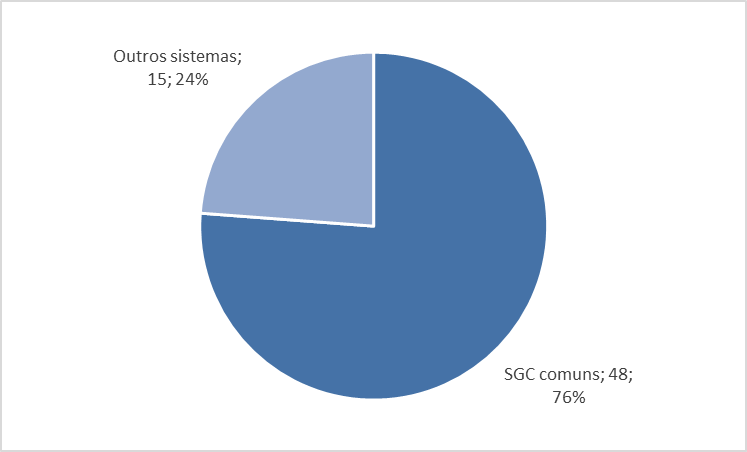
\includegraphics[width=0.7\textwidth]{figuras/adocao-de-cms}
 
 \label{cms-universidade-opcao}
 \fonte{\citeonline{elias}.}
\end{figure}

\begin{figure}[htb]
 \centering
 \caption{Tipos de CMSs adotados pelas universidades federais}
 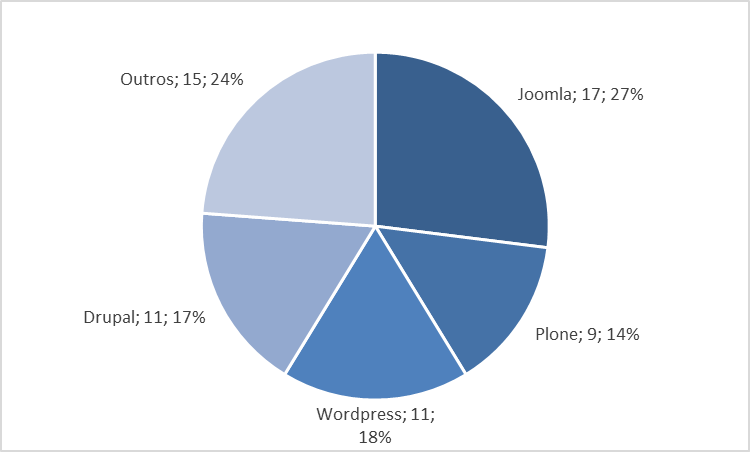
\includegraphics[width=0.7\textwidth]{figuras/tipos-de-cms}
 
 
 \fonte{\citeonline{elias}.}
 \label{cms-universidade-adocao}
\end{figure}

\newpage
Após as observações anteriores, serão comparados os quatro sistemas predominantes com o objetivo de avaliá-los e determinar qual deles possui o melhor resultado geral diante das seguintes métricas: desempenho geral, comércio eletrônico, aplicações integradas, flexibilidade, interoperabilidade, gerenciamento, performance, facilidade de uso, suporte e segurança. As Figuras \ref{drupal}, \ref{joomla}, \ref{plone} e \ref{wordpress} referem-se ao desempenho obtido pelo respectivo sistema para cada uma das métricas propostas. Por fim, a Figura \ref{desempenho-geral} demonstra o desempenho geral obtido por cada um.

\newpage

\begin{figure}[htb]
 \centering
 \caption{Desempenho obtido pelo \textit{Drupal}}
 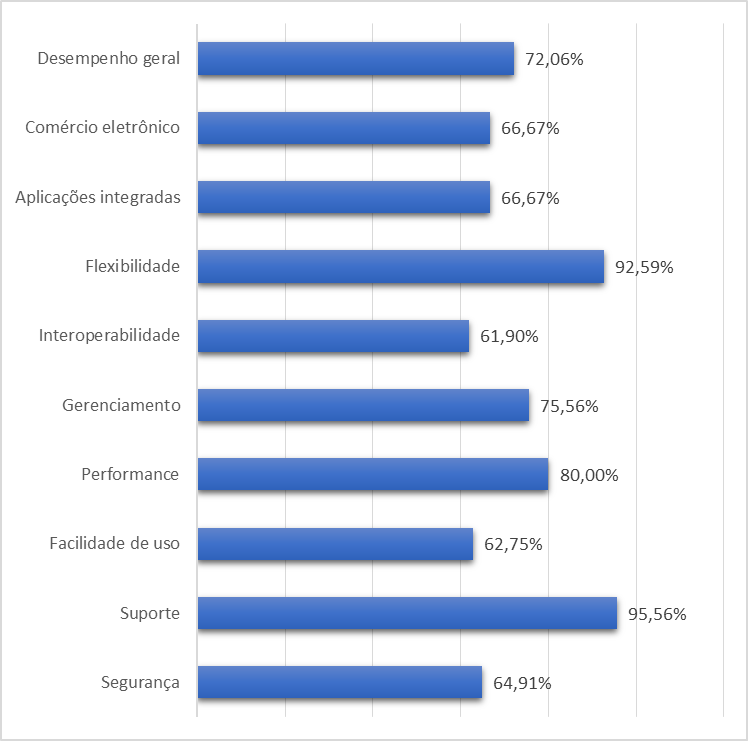
\includegraphics[width=0.7\textwidth]{figuras/desempenho-drupal}
 \label{drupal}
 \fonte{\citeonline{elias}.}
\end{figure}

Diante do que foi apresentado na Figura \ref{drupal}, os recursos que mais se destacam positivamente no \textit{Drupal} são a flexibilidade (92,59\%), performance (80\%) e suporte (95,56\%), e negativamente: interoperabilidade (61,9\%), facilidade de uso (62,75\%) e segurança (64,91\%). Significando que o gerenciador possui um alto grau de customização, rapidez e comunidade de apoiadores, porém peca na segurança das informações, na diminuição da curva de aprendizado dos usuários e na integração a outras tecnologias.
\newpage

\begin{figure}[htb]
 \centering
 \caption{Desempenho obtido pelo \textit{Joomla!}}
 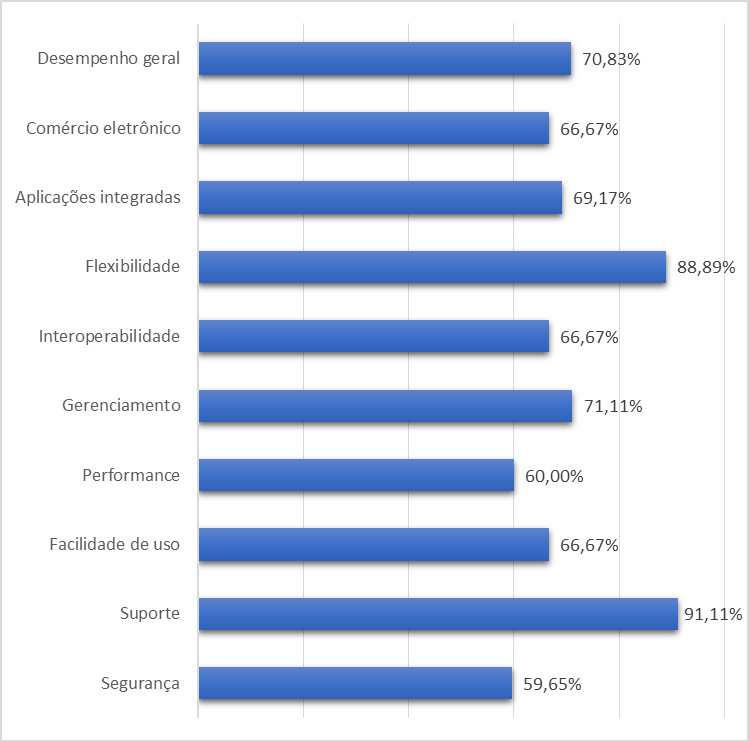
\includegraphics[width=0.7\textwidth]{figuras/desempenho-joomla}
 \label{joomla}
 \fonte{\citeonline{elias}.}
\end{figure}

Analisando as características do \textit{Joomla!} através da Figura \ref{joomla}, é possível identificar duas grandes qualidades: a flexibilidade (88,89\%) e o suporte (91,11\%), enquanto que suas maiores limitações se concentram intensamente na performance (60\%) e segurança (59,65\%). Ele aparenta ser mais regular que o CMS anterior, visto que são poucas as métricas em que obteve desempenho fora do intervalo de 60\% a 71\%.   
\newpage
\begin{figure}[htb]
 \centering
 \caption{Desempenho obtido pelo \textit{Plone}}
 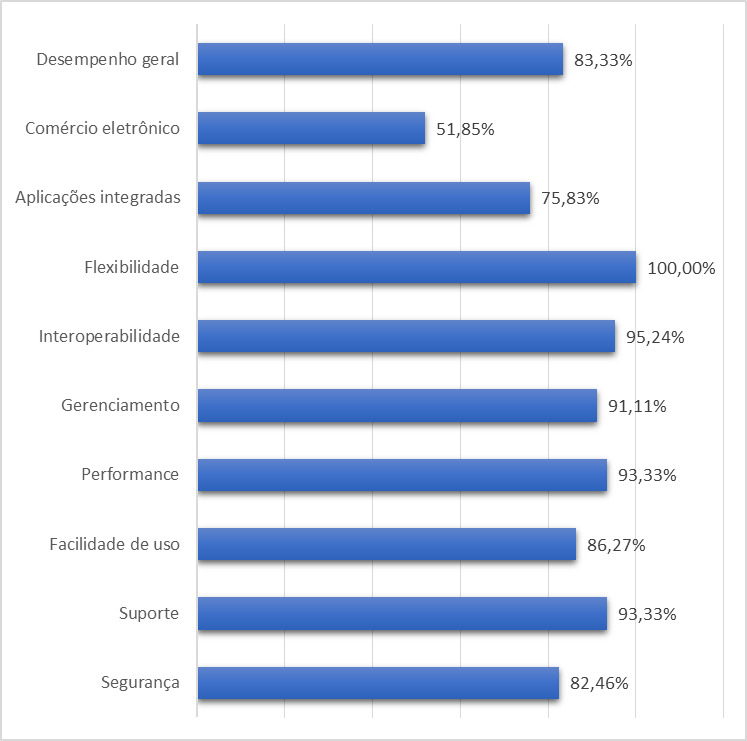
\includegraphics[width=0.7\textwidth]{figuras/desempenho-plone}
 \label{plone}
 \fonte{\citeonline{elias}.}
\end{figure}

Com resultados muito distintos dos obtidos anteriormente, o \textit{Plone} alcançou altíssimo desempenho em diversas métricas, obtendo mais de 90\% em 5 delas, com destaque maior para a flexibilidade (100\%) e a interoperabilidade (95,24\%). Em contrapartida, analisando ainda a Figura \ref{plone}, sua avaliação referente a comércio eletrônico foi extremamente baixa, alcançando somente (51,85\%) de desempenho neste quesito. 
\newpage

\begin{figure}[htb]
 \centering
 \caption{Desempenho obtido pelo \textit{WordPress}}
 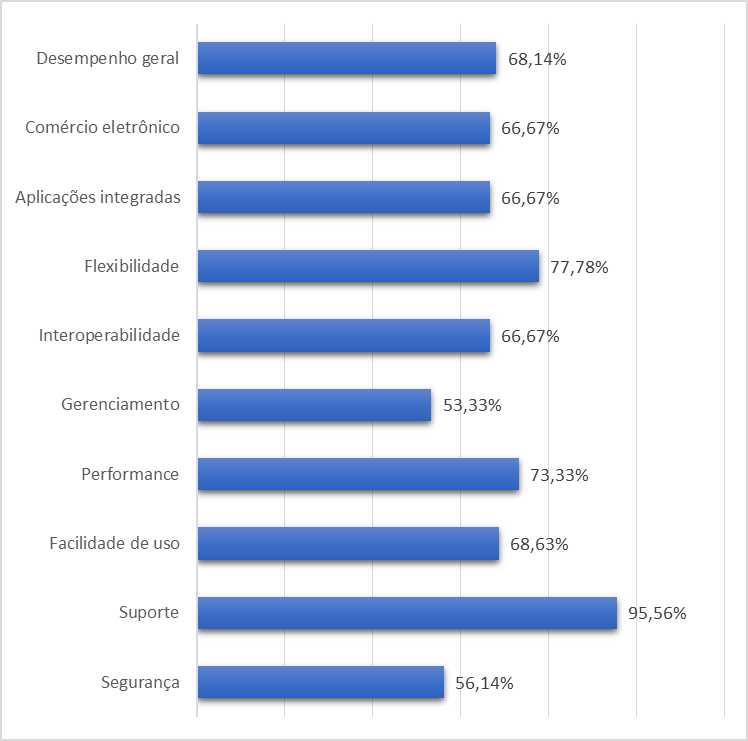
\includegraphics[width=0.7\textwidth]{figuras/desempenho-wordpress}
 \label{wordpress}
 \fonte{\citeonline{elias}.}
\end{figure}

Com uma regularidade aproximada à do \textit{Joomla!}, a Figura \ref{wordpress} demonstra que o \textit{WordPress} adquiriu desempenho bem aproximado em diversos aspectos, com uma variação maior em flexibilidade (77,78\%) e suporte (95,56\%), e uma baixa avaliação em gerenciamento (53,33\%) e segurança (56,14\%). Tais dados demonstram a similaridade entre os gerenciadores \textit{Joomla!} e \textit{WordPress} e o porquê deste ser amplamente usado, dado seu suporte e flexibilidade de integração com outras ferramentas. Porém sua segurança e gerenciamento são pouco apreciadas, principalmente em gerenciamento, que diz respeito a gestão de publicidade, prancheta, gerenciamento de tradução e diversos outros aspectos, que podem ser conferidos em \citeonline[~p. 70]{elias}.   
\newpage

\begin{figure}[htb]
 \centering
 \caption{Desempenho geral obtido pelos sistemas}
 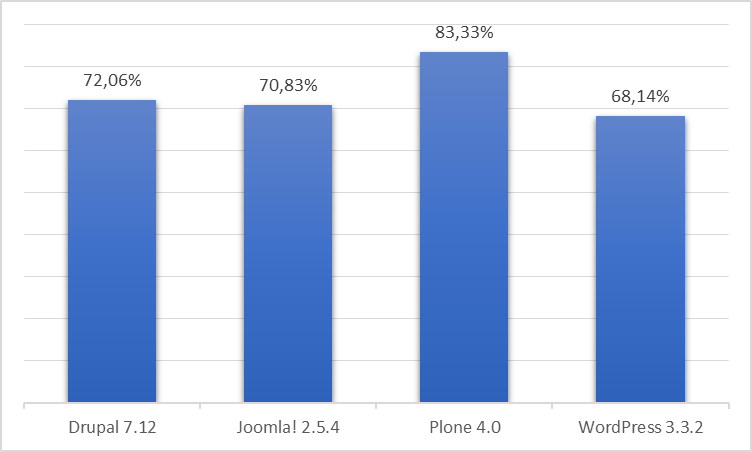
\includegraphics[width=0.7\textwidth]{figuras/desempenho-geral-cms}
 \label{desempenho-geral}
 \fonte{\citeonline{elias}.}
\end{figure}


Então pode-se considerar, diante do desempenho geral apresentado na Figura \ref{desempenho-geral} e dos testes executados cujos resultados estão exibidos nas figuras de desempenhos individuais, que o \textit{Plone} é o mais balanceado em termos de aspectos negativos e positivos, fornecendo uma maior confiança aos desenvolvedores de sistemas web que precisam de sistemas que reajam bem a módulos mais robustos, que sejam seguros e com grande comunidade virtual para auxílio ao desenvolvimento.

A Figura \ref{uso-plone-mercado} mostra uma análise de posicionamento de mercado dos CMSs mais usados no mundo:

\begin{figure}[htb]
 \centering
 \caption{Análise de posicionamento de mercado com destaque para o \textit{Plone}}
 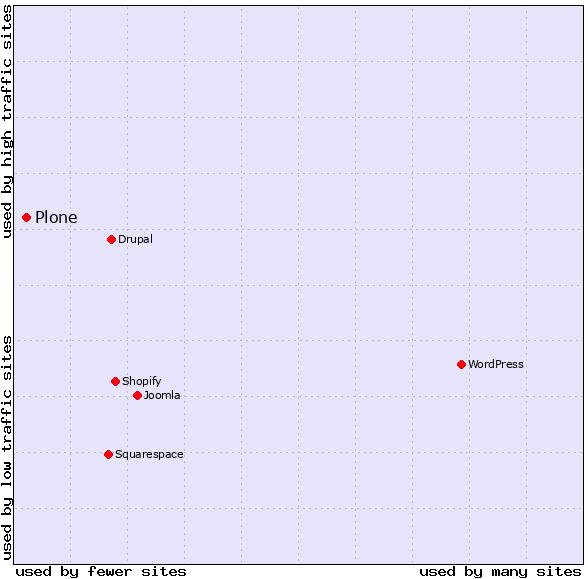
\includegraphics[width=0.7\textwidth]{figuras/cms_mercado}
 
 \label{uso-plone-mercado}
 \fonte{\apud{plonemercado}{elias}.}
\end{figure}

\newpage

Através da Figura \ref{uso-plone-mercado} percebemos que o \textit{Plone} é muito preferido em situações que envolvem sistemas que receberão grande número de requisições de visitantes e usuários.

Outro fator importante a se destacar é a baixa adesão das pessoas a esse CMS. Pela figura percebe-se que o \textit{WordPress}
é disparadamente o sistema mais utilizado, e o \textit{Plone}, o que está em menor número de sites.

O \textit{Idealware}, um site que tem o propósito de ajudar organizações sem fins lucrativos a tomar decisões inteligentes sobre tecnologia, publicou o seguinte artigo: \textit{Consumers Guide to Open Source Content Management Systems for Nonprofits: Comparing WordPress, Drupal, and Plone}, detalhando todos estes três sistemas.

Para a comparação, houve a criação da Tabela \ref{nivel-cms} contendo 15 atributos, na qual está atribuído o nível dos softwares para cada um deles, sendo 1 significando um nível ruim de satisfação, 2 significando um nível médio e 3, por sua vez, determinando que o sistema de gerenciamento cobre muito bem tal aspecto.

\newpage

\begin{table}[h]
\centering
\scalefont{0.7}
\caption{Nível de satisfação do CMS por requisito}
\vspace{0.5cm}

\setlength{\extrarowheight}{0.25cm}
\begin{tabular}{l|c|c|c}
 
\textbf{Requisito} & \textbf{\textit{Drupal}} & \textbf{\textit{Plone}} & \textbf{\textit{WordPress}} \\ % Note a separação de col. e a quebra de linhas
\hline                               % para uma linha horizontal
Facilidade de hospedagem e instalação & 3 & 1 & 3 \\
Facilidade de configurar um site simples & 3 & 3 & 3 \\
Curva de aprendizado para configurar um site complexo & 2 & 1 & 3 \\
Facilidade edição de conteúdo & 3 & 3 & 3 \\
Facilidade de gerenciar um site & 2 & 2 & 3 \\
Flexibilidade estrutural & 3 & 3 & 2 \\
Flexibilidade gráfica & 3 & 3 & 3 \\
Flexibilidade de suporte móvel & 3 & 3 & 3 \\
Integração com dados constituintes & 2 & 2 & 1 \\
Funções de usuário e fluxo de trabalho & 2 & 3 & 2 \\
Comunidade/Funcionalidade na Web 2.0 & 3 & 2 & 3 \\
Acessibilidade & 3 & 3 & 2 \\
Otimização para mecanismos de pesquisa & 2 & 3 & 2 \\
Estendendo além da funcionalidade existente & 3 & 3 & 3 \\
Apoio e força da comunidade & 3 & 3 & 3 \\
\hline   
\end{tabular}
\fonte{\citeonline{idealware-cms}. Adaptado.}
\label{nivel-cms}
\end{table}


A Tabela \ref{nivel-cms} expressa uma informação importante: o \textit{Plone} proporciona pouca facilidade para hospedagem, instalação e uma baixa curva de aprendizado por parte do desenvolvedor ao se deparar com a construção de um site complexo. Tais fatores associados à baixa popularidade do mesmo em relação ao outros sistemas o torna menos acessível aos usuários, impactando diretamente no número de sites que o utilizam.

Essas desvantagens se tornam pouco relevantes ao se considerar que a pessoa responsável pela implantação do sistema é capacitada para desempenhar a tarefa, além de que a aplicação poderá ou não ser complexa. Logo, é necessária a realização de um estudo de caso para avaliar se realmente compensa a utilização do \textit{Plone} para a construção de um sistema web, observando as vantagens e desvantagens anteriormente mencionadas. 

\hspace{2.5cm}

\section{Servidor Virtual Privado}
\label{sec:vps}

\hspace{2.5cm}

Os Servidores Virtuais Privados (VPS) surgiram em decorrência da continuação do processo de virtualização de máquinas. Com a VPS é possível ter sua própria máquina hospedada na nuvem, porém, assim como na Máquina Virtual (VM), o seu responsável não possui acesso direto ao hardware, somente ao software.

Segundo \citeonline{chuchuca2016implementacion} a hospedagem VPS é ideal para quem possui demandas que podem ser satisfeitas de forma compartilhada, mas desejando pagar menos que na contratação de um servidor dedicado. Uma curiosidade sobre a VPS é a permissão de gerenciar o software de uma máquina inteira, inclusive no que diz respeito a configuração de servidores locais. 

Esse tipo de serviço requer maior responsabilidade e conhecimento do administrador da máquina, pois ele deve entender o funcionamento e divisão da mesma dependendo de seu sistema operacional, e ainda seus detalhes técnicos e comandos de configuração e conexão via SSH. Em relação à segurança, \citeonline{elizabeth2017diseno} revelam este ser um fator positivo para os Servidores Privados Virtuais. Para isso, ela faz menção aos sistemas VoIP e às máquinas físicas, que são mais propensos a ataques, ameaças e riscos principalmente no caso de máquinas físicas, que estão sujeitas a blecautes, curto-circuitos, dano no dispositivo ou ainda a roubo de informações. Um outro problema em relação aos servidores físicos está na compatibilidade entre hardware e software, pois todos os equipamentos da máquina devem ser compatíveis. Esses transtornos não são encontrados na VPS, visto que a própria empresa que oferece o serviço de hospedagem já é responsável por manter a compatibilidade dos elementos e a segurança da máquina.  


% \hspace{2.5cm}
% 
% \section{Testes de Software}
% \label{sec:testessoftware}
% %Testes de software
% \hspace{2.5cm}
% 
% Vou deixar po último porque não sei se vai dar tempo de executar.


\hspace{2.5cm}
\section{Ferramentas}
\label{sec:ferramentas}

\hspace{2.5cm}

Nesta seção, o objetivo será a junção e uma explicação sucinta das ferramentas utilizadas no processo de desenvolvimento e avaliação do sistema web.  


%JMetter

% \textbf{\textit{Apache JMeter}}: é uma ferramenta capaz de realizar testes em aplicações web. Por ser desenvolvido em Java, 
% ela é também multiplataforma, ou seja, pode ser executada em vários sistemas operacionais. Um teste típico com o \textit{JMeter} envolve o envio
% de requisições a uma aplicação através de um \textit{loop}, cujo limite de laços e número de requisições são definidos pelo usuário.

% \begin{figure}[htb]
%  \centering
%  \caption{Tela inicial do \textit{Apache JMeter}}
%  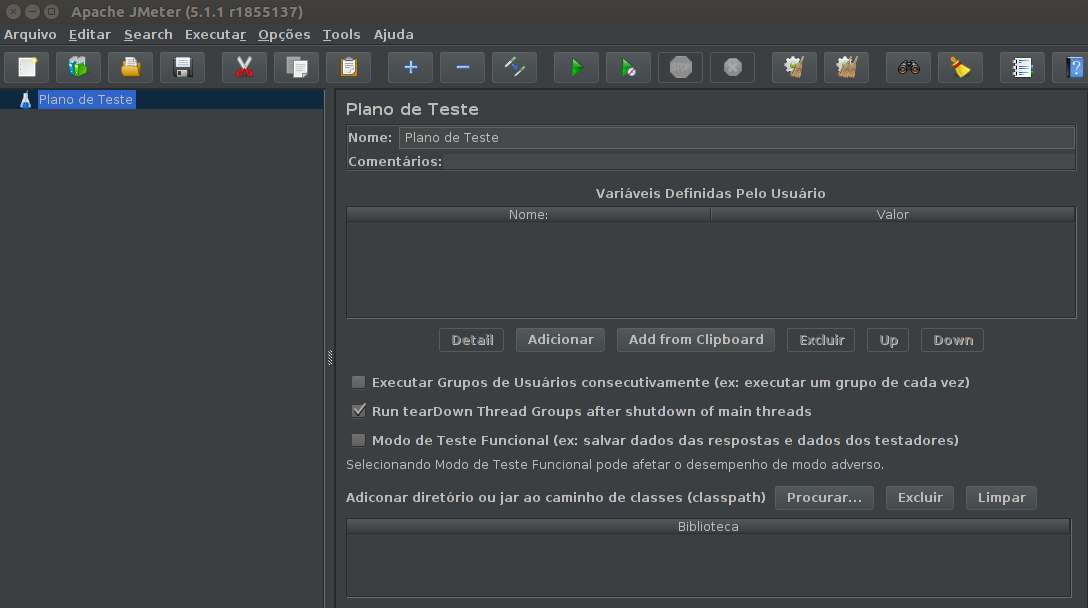
\includegraphics[width=0.7\textwidth]{figuras/jmeter}
%  
%  \label{jmeter}
%  \fonte{Autor.}
% \end{figure}

%Plone
\textbf{\textit{Docker}}: é uma tecnologia ligada à infraestrutura de máquinas. Surgiu em 2013 após a mudança do nome \textit{dotCloud} para o atual. O \textit{Docker} usa a ideia de ``camadas'' e \textit{containers}. \textit{Containers} são aplicações que utilizam o mesmo \textit{kernel} do sistema operacional onde está rodando. Uma aplicação pode ser praticamente qualquer software, inclusive outro sistema operacional, desde que tenha uma ``imagem'' para ela, porque um \textit{container} é executado a partir de uma imagem.

Alguns podem confundí-lo com Máquinas Virtuais (VMs), mas no livro de \citeonline{vitalino2016descomplicando}, os autores deixam claro as suas diferenças. Na Máquina Virtual, o sistema operacional a ser virtualizado é inicializado carregando todo o seu hardware e mais recursos que os da máquina \textit{host}, diferentemente dos \textit{containers}, que utilizam os mesmos recursos da máquina hospedeira, havendo, assim, um ganho em desempenho em relação à VM.

Compreender o conceito de \textit{containers} é fundamental para entender o conceito de camadas, isto porque eles são formados por \textit{layers} (camadas). Essa ideia parte do princípio de compartilhamento e reutilização, visto que vários \textit{containers} podem compartilhar camadas subjacentes, diminuindo o uso de recursos \cite{prada4docker}. A Figura \ref{containers} esquematiza a estrutura da arquitetura de \textit{containers} e camadas.

\newpage

\begin{figure}[htb]
 \centering
 \caption{Esquema explicativo da estrutura de \textit{containers}}
 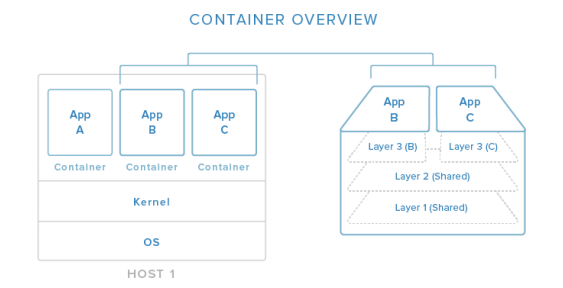
\includegraphics[scale=0.6]{figuras/containers}
 
 \label{containers}
 \fonte{\cite{prada4docker}.}
\end{figure}

Entre as diversas vantagens que o \textit{Docker} proporciona podemos citar a teoria da escalabilidade, que corresponde à segmentação de todo um sistema, sua divisão em partes realiza o carregamento parcial dos \textit{websites} contribuindo para a diminuição do tempo de acesso do visitante à página web. Tal modularização também auxilia na manutenção e disponibilidade das partes, isto porque, dependendo da situação, \textit{containers} podem estar funcionando normalmente mesmo que um deles esteja em manutenção ou tenha sido derrubado, possibilitando ao usuário acessar um componente desde que o mesmo não dependa do inacessível. 

Também é importante mencionar que com a correta orquestração dos \textit{containers}, os mesmos poderão ser inseridos em uma imagem, através do recurso do \textit{Docker Compose}, e carregados em qualquer ambiente, desde que ele possua o \textit{Docker}. Esta funcionalidade garante o princípio de portabilidade e faz com que um sistema inteiro funcione em várias máquinas e sistemas operacionais com apenas os comandos de importar a imagem e iniciar um \textit{container} da mesma.

Ainda pelo \textit{Docker} é possível verificar o comportamento e eventuais problemas relacionados aos \textit{containers} através de seus \textit{logs}.

%Git
\textbf{\textit{Git}}: é um sistema de versionamento de código lançado em 2005. O controle de versão possibilita acompanhar o desenvolvimento de um
software sem alterar a versão principal, restaurar uma determinada versão anterior e até compartilhar o mesmo código com outros desenvolvedores \cite{palestinoestudo}. ``O Git possui uma ênfase em velocidade, integridade dos dados e suporte para \textit{workflows} não lineares e distribuídos'' \cite[p. 10]{ghezzi2015api}.

Para hospedar códigos do \textit{Git} existem diversos sites, porém o mais usado e também um dos poucos que oferecem opções de hospedagem pública e privada é o \textit{GitHub}, que em 2019, inclusive, tornou possível aos usuários a criação de repositórios privados gratuitamente, o que antes, segundo \citeonline{chacon2010pro}, era uma funcionalidade paga. 

%Analytics
\textbf{\textit{Google Analytics}}: é uma ferramenta da Google utilizada para obtenção de relatórios sobre número, origem, tempo de duração e muitas outras informações sobre as visitas que um sistema recebe. Com ela é possível identificar padrões relacionados a essas visitas, taxa de aumento ou diminuição no número de visitantes, páginas da aplicação mais acessadas, entre outros dados. 

%MySQL
\textbf{MySQL}: a SQL (Linguagem de Consulta Estruturada, em português) é um tipo de programação especializada em trabalhar com bancos de dados relacionais \cite[~p. 7, tradução nossa]{mysql2001mysql}. Um dos diversos bancos de dados relacionais existentes é o MySQL, desenvolvido pela empresa Microsoft e considerado um servidor e gerenciador de banco de dados (SGBD) relacional de código aberto (\textit{open source}). O MySQL possui todos os atributos necessários a um banco de dados de grande porte e é reconhecido por muitos como o \textit{open source} mais concorrente de SGBDs de código fechado \cite{milani2007mysql}.


\hspace{2.5cm}

\hspace{2.5cm}
\section{Estado da Arte}
\label{sec:trabalhoscorrelatos}
\hspace{2.5cm}

A presente seção visa apresentar trabalhos desenvolvidos por outros pesquisadores que envolvam a concepção de sites ou sistemas para associações, centros educacionais ou demais instituições sem fins lucrativos. Com esse objetivo, duas pesquisas foram selecionadas, ambas dissertações para obtenção do grau de mestre em suas respectivas áreas. 

A busca por ferramentas desenvolvidas por profissionais ou estudantes de TI para associações não obteve os resultados esperados, logo as pesquisas a serem estudadas foram contruídas por estudantes que buscavam o grau de mestre em outras áreas tecnológicas, sendo elas de Assessoria de Administração, no Instituto Superior de Contabilidade e Administração do Porto (ISCAP), e de Ciências, na Universidade Federal Rural do Rio de Janeiro (UFRRJ). A seguir, as pesquisas serão demonstradas na sequência em que foram mencionadas anteriormente. 

\hspace{2.5cm}
\subsection{Pesquisa correlata: Concepção e Implementação de um Website de uma Associação Sindical}
\hspace{2.5cm}

O estudo tem como público alvo o Sindicato Nacional dos Trabalhadores da Industria e Comércio de Alimentação, Bebidas e Afins (SINTICABA), localizado em Portugal, como será apresentado mais adiante. A autora, \citeonline{moreno2012concepccao}, explica que para o projeto ``é esperado conceber uma ferramenta de comunicação que acompanhe as tecnologias de informação e comunicação'', também atendendo às necessidades tanto por parte de associados como do próprio sindicato. A interatividade e a difusão da informação são também objetivadas, desde que não dependam de um suporte físico ou temporal.

O SINTICABA é uma associação sindical localizada na cidade de Porto, em Portugal, e surgiu no ano de 2000. Ela é financiada por cerca de 650 trabalhadores sindicalizados e suas principais atividades são: 

\begin{citacao}
Apoio jurídico aos sócios, formação profissional, fiscalizar e reclamar a aplicação das leis do trabalho e das convenções coletivas de trabalho, negociação da contratação coletiva dos diversos setores de atividade que representa, prestar assistência jurídica e judiciária aos associados nos conflitos resultantes de relações de trabalho e intervir nos processos disciplinares instaurados aos associados \apud[~p. 31]{estatutos}{moreno2012concepccao}.
\end{citacao}

O sindicato é composto por três órgãos principais, como se segue:

\begin{enumerate}
 \item \textbf{Mesa da Assembleia Geral}: ``órgão deliberativo, é responsável pela condução dos trabalhos e pela sua secretaria, sendo composta por um presidente, dois vice-presidentes e dois suplentes'' \apud[~p. 33]{estatutos}{moreno2012concepccao};
 \item \textbf{Direção}: dentre outros deveres, este órgão é responsável pela execução das deliberações tomadas pela Assembleia Geral, apresentação à esta do relatório de contas e orçamento para o ano subsequente, e representação do sindicato em eventos de natureza jurídica ou social. Fazem parte dele um presidente e seu vice, um secretário, um tesoureiro, três vogais e dois suplentes \apud[~p. 33]{estatutos}{moreno2012concepccao}; e
 \item \textbf{Conselho Fiscal}: por ser um órgão fiscalizador a ele se compete: examinar documentos, contas e relatórios, além de se posicionar sobre tais objetos analisados. Ele é composto por um presidente, um secretário e um relator \apud[~p. 34]{estatutos}{moreno2012concepccao}. 
\end{enumerate}

O trabalho desenvolvido pela autora teve como motivação a utilidade de estabelecer uma comunicação mais fluida entre associado e sindicato, mais rápida e com menos custos, seja com deslocamentos, contas vinculadas à utilização de telefones e correios. Antes da implementação do site os sócios dependiam de telefonemas, fax, um delegado sindical ou até mesmo de se deslocarem para solicitar informações relacionadas às atribuições da associação. Pensando nisso foram realizados uma entrevista e um questionário, este com um total de 250 respostas obtidas, sobre as funcionalidades que a ferramenta tecnológicas deveria englobar, obtendo-se o seguinte resultado, segundo \citeonline{moreno2012concepccao}:

\begin{itemize}
 \item fazer inscrição de sócios;
 \item atualizar dados pessoais;
 \item inserir perguntas de caráter jurídico;
 \item inserir perguntas de caráter geral; e
 \item dar sugestões ou fazer comentários.
\end{itemize}

A ferramenta escolhida pela autora para o desenvolvimento do site fora basicamente um Sistema de Gerenciamento de Conteúdo já mencionado nesse trabalho, o \textit{Joomla!}. Para a autora, \citeonline{moreno2012concepccao}, a seleção desta ferramenta se justifica pelo fato de, segundo ela, ser de simples para manipulação e não exigir conhecimentos sobre programação, atribuindo-lhe ainda a característica de ser um dos melhores gestores de conteúdo.

O domínio escolhido foi: \textit{sinticaba.com}, sua escolha foi esclarecida pela economia e redução da burocracia em alugar o endereço eletrônico. A fim de antecipar detalhes do trabalho para futuras comparações, vale ressaltar que em momento algum do trabalho a autora cita a adoção de qualquer metodologia de desenvolvimento de software.

Após a disponibilização do site na internet, o mesmo foi divulgado através de convites enviados via e-mail e cartas para todos os associados com o intuito de que visitassem o site dessem suas opiniões através de um formulário presente na página inicial, disponível na Figura \ref{pagina-inicial-sindicato}.

\begin{figure}[htb]
 \centering
 \caption{Página inicial do site da Sinticaba}
 
\includegraphics[width=0.7\textwidth]{figuras/pInicial-Sindicato}
 \fonte{\citeonline{moreno2012concepccao}.}
 \label{pagina-inicial-sindicato}
\end{figure}


Ao final do trabalho, foi ressaltada a importância de se manter o site sempre atualizado, já que a etapa concluída é somente o ponto de partida para a construção da ferramenta, que possivelmente, poderá ficar ainda mais completa e repleta de funcionalidades além das implementadas. 

Como trabalhos futuros, segundo ela, a elaboração de um manual técnico que explique as funcionalidades do site para o presidente da associação, que é quem fará a manutenção e a atualização das informações, deve ser efetivada. Também está prevista a coleta de mais sugestões e questões levantadas pelos associados, visto que até o término do projeto a avaliação do site por parte dos associados ainda não havia sido efetuada, além da atualização do sistema de gestão de conteúdo \textit{Joomla!} sempre que for lançada uma nova versão do software.


\hspace{2.5cm}
\subsection{Pesquisa correlata: Construção Coletiva do Portal Educação do Campo}
\hspace{2.5cm}

A pesquisa partiu de observações e questionamentos gerados ao longo de seis anos, enquanto o autor, \citeonline{soares2017construccao}, foi docente em Agricultura e Zootecnia, no Centro Estadual Integrado de Educação Rural de Boa Esperança (CEIER/BE), estado do Espírito Santo. Os sujeitos presentes na pesquisa foram do corpo docente, que ofertava ``140 vagas para o ensino fundamental do 6° ao 9° ano e 90 vagas para o ensino médio integrado ao curso técnico em meio ambiente'' \cite{soares2017construccao}.

As motivações para a realização da pesquisa, citadas pelo autor, são compreendidas como as seguintes: 

\begin{itemize}
 \item dificuldades ao disponibilizar materiais didáticos para as aulas, como textos, imagens e vídeos, aos estudantes e professores;

 \item aumento no tamanho ocupado pelos materiais por estarem sendo armazenados em um único local, compreendendo também em risco de perda de conteúdo ou por defeito físico do disco rígido ou por influência de vírus ou fator semelhante; e
 
 \item falta de uma biblioteca específica para modalidade educação do campo, que poderia facilitar ``o acesso a bibliografia e outros recursos didáticos que tem como ideologia o desenvolvimento da agroecologia e da agricultura familiar'' \cite{soares2017construccao}.
\end{itemize}

Os objetivos específicos do trabalho são: entender como funcionam sites e portais educacionais, analisar as especificações da modalidade de educação no campo e das disciplinas diversas do CEIER de Boa Esperança, e construir e avaliar um portal educacional e suas características pedagógicas \cite{soares2017construccao}.

A coleta de requisitos para o portal educacional foi concebida por meio de uma reunião de apresentação e explicação dos objetivos do portal aos professores, reunindo um grande conjunto de sugestões pertinentes a sua concepção. Assim sendo, obteve-se alguns requisitos para o portal que estão, em maioria, citados adiante. Entre outras peculiaridades e segundo o autor, o portal deve ser capaz de:

\begin{itemize}
 \item possuir design e recursos multimídias, como áudio e vídeo, que auxiliem no cotidiano da agricultura familiar e no desenvolvimento da agroecologia;
 \item possuir domínio que esteja de acordo com as características da modalidade educação do campo, auxiliando na identificação dos seus objetivos;
 \item ``fornecer notícias e ferramentas necessárias ao cotidiano do meio rural, como o calendário agrícola, previsão do tempo, estratégias contra a seca, fases da lua, etc'' \cite{soares2017construccao};
 \item ser de rápido acesso e carregamento de páginas; e
 \item possuir interação entre usuários e redes sociais.
\end{itemize}

Ainda em relação aos objetivos da plataforma, o autor ressalta que o portal da Educação do Campo terá caráter meramente informativo e reunirá somente informações pertinentes à essa modalidade. Na hospedagem e implementação do portal, optou-se pelo servidor UOL \textit{Host}, que segundo o autor, oferece maior segurança ao hospedar a aplicação. O domínio foi escolhido de acordo com os objetivos do portal, sendo ele: \textit{http://www.educacaodocampo.com.br/} e a ferramenta construtora de sites, assim como a hospedagem, pertence ao UOL \textit{Host}, tal escolha foi embasada na possibilidade de usuários leigos em linguagens de programação conseguirem manter seus \textit{websites} através dessa ferramenta.

Após o término da implementação do portal, o autor buscou formas eficientes de divulgação do mesmo, chegando à conclusão de que a utilização do Facebook foi determinante. Segundo ele, a sua conexão do portal a um perfil na rede social ``se tornou rapidamente a alternativa mais eficiente de visualização, divulgação e aquisição de material midiático''. A página inicial do portal está representada na Figura \ref{pagina-inicial-portal}.

\begin{figure}[htb]
 \centering
 \caption{Página inicial do portal Educação do Campo}
 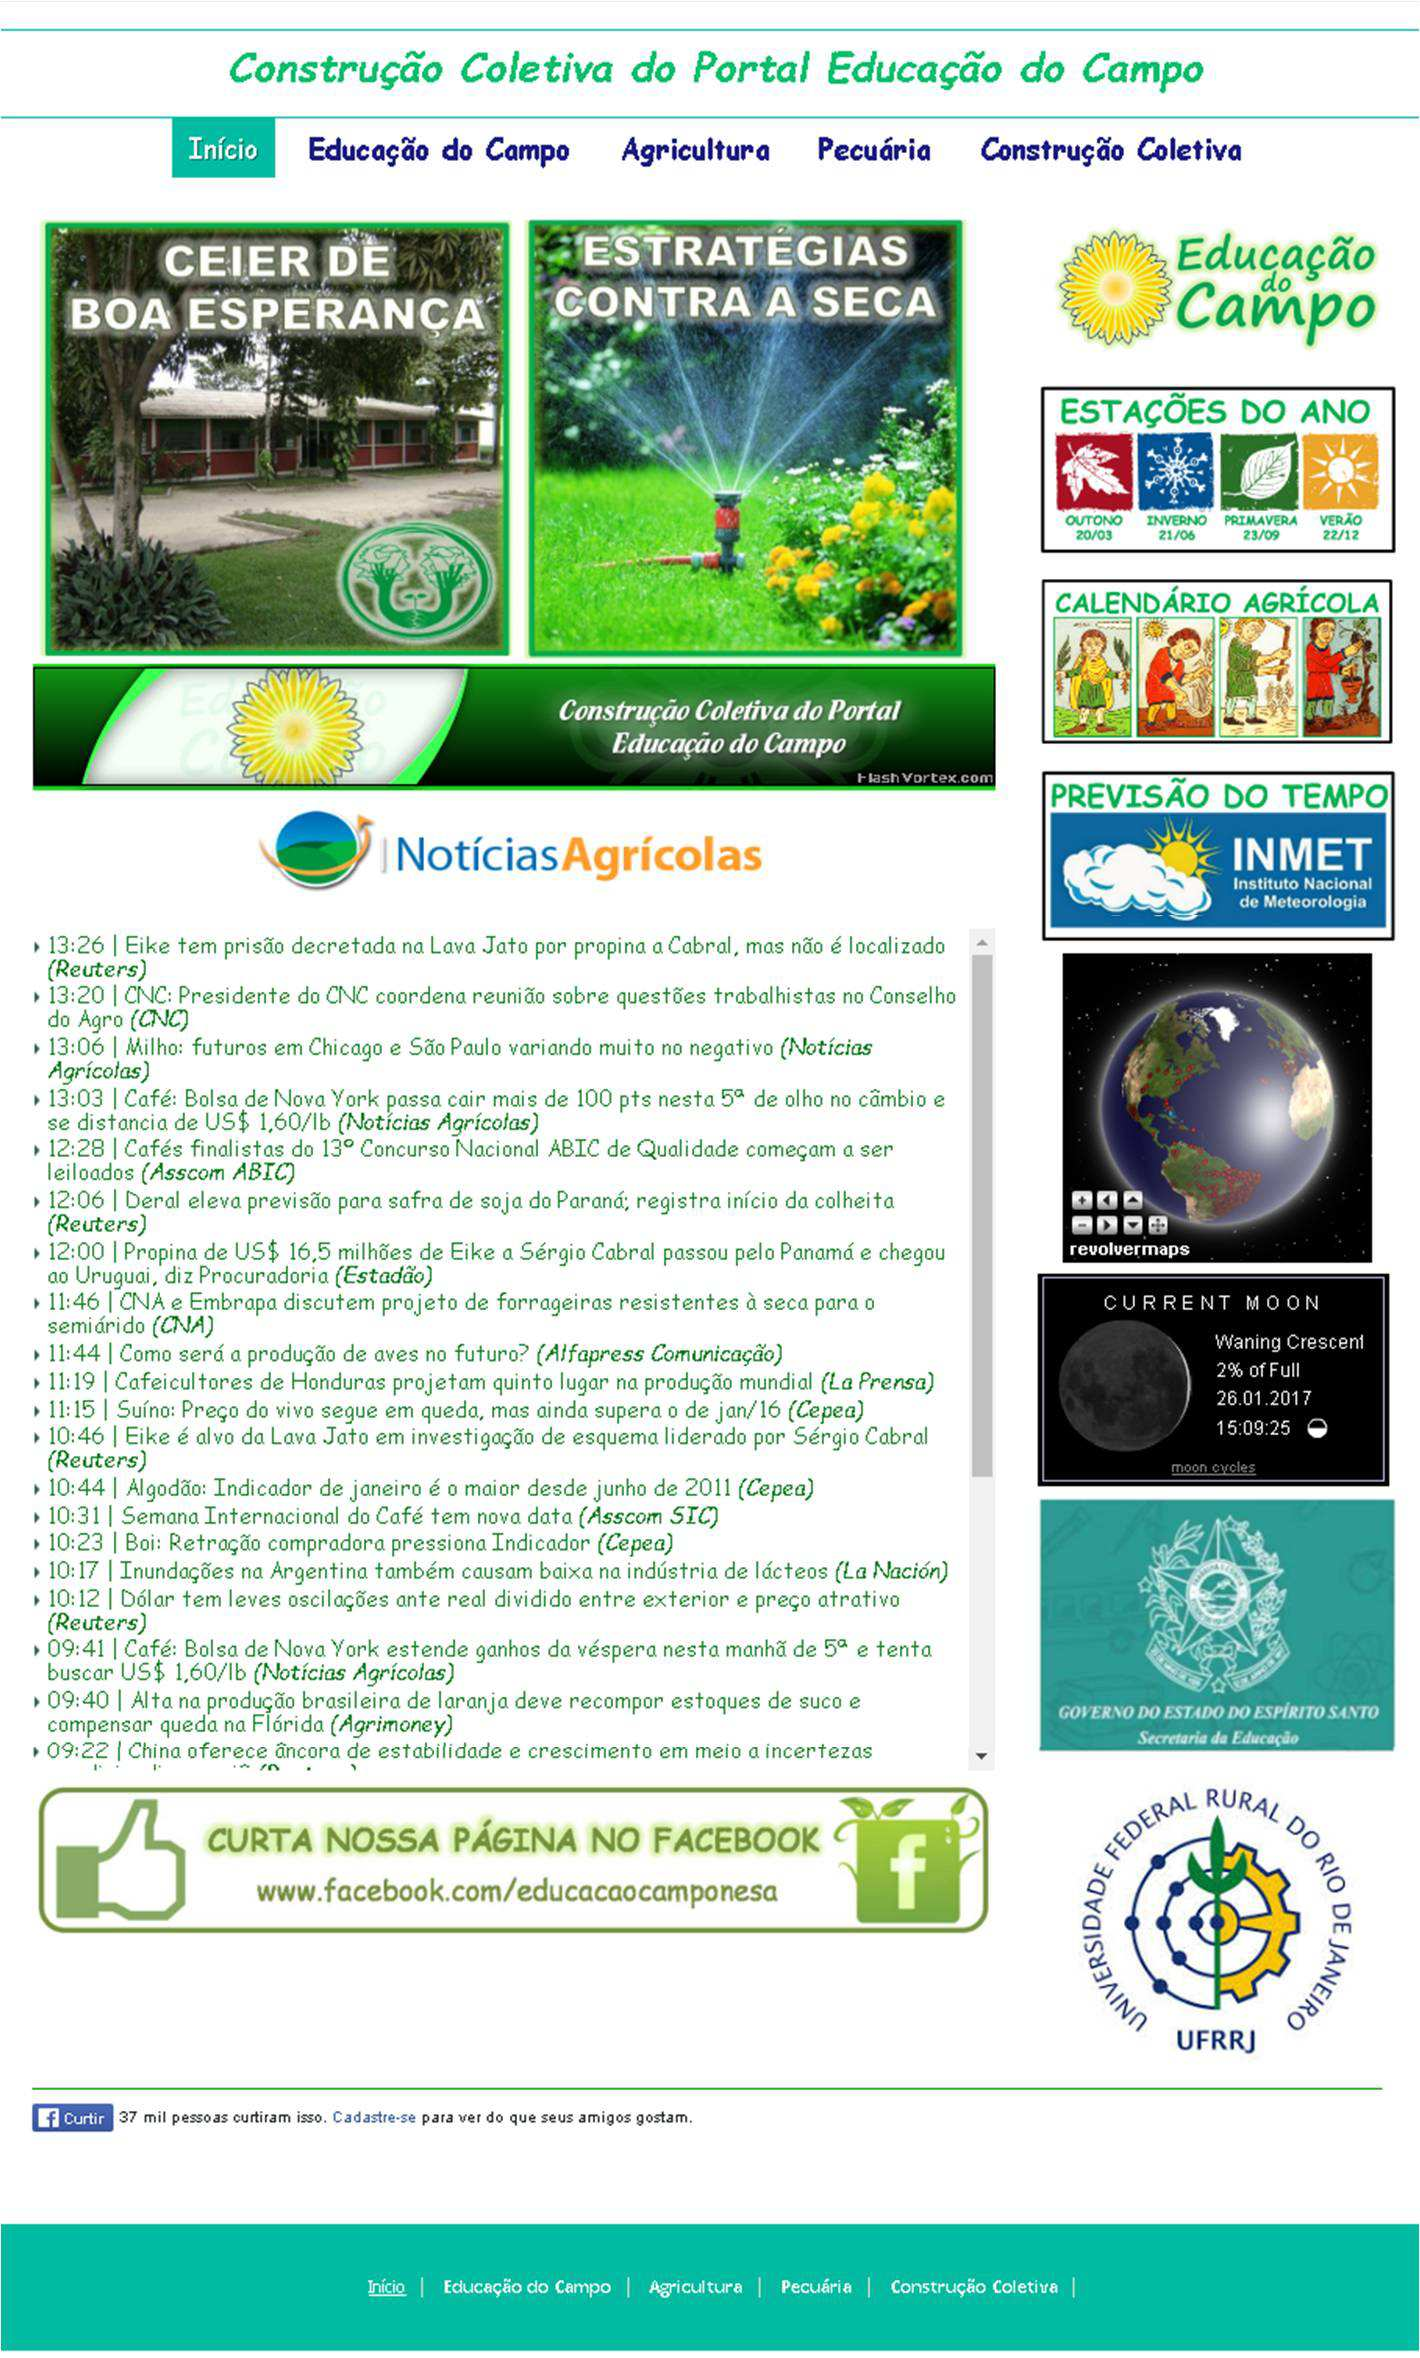
\includegraphics[width=0.6\textwidth]{figuras/pInicial-Centro}
 \fonte{\citeonline{soares2017construccao}.}
 \label{pagina-inicial-portal}
\end{figure}

\newpage

As conclusões encontradas por \citeonline{soares2017construccao} foram que a taxa de aprovação entre os professores para a usabilidade e o conteúdo pedagógico do portal foi de 85,5\% e as principais deficiências encontradas na utilização do portal, que devem ser revisadas, se encontram a seguir:

\begin{citacao}
 Utilização do portal educacional na escola; utilização nas séries finais do ensino fundamental; utilização no ensino médio e profissionalizante; utilização na sala de aula com o auxílio de smartphones ou tablets; utilização no laboratório de
informática educativa; auxiliar na aprendizagem e compreensão de determinados conteúdos e reforçar algumas habilidades que não sejam na frente do computador \cite{soares2017construccao}. 
\end{citacao}

A instabilidade na quantidade de visitantes também foi um fator considerável, visto que nos primeiros três meses após a implementação do portal, foram contabilizados 150 visitantes, já no trimestre seguinte foram notados 14052, indicando 74\% de todas as visitas registradas durante os doze primeiros meses. Em contrapartida ao alto crescimento no segundo trimestre, foram obtidas, no segundo semestre, pouco mais de 25\% de todas as visitas registradas ao longo do ano. Segundo o autor, tal variação se deve ao fato de não se ter investimento em publicidade no Facebook, mesmo com a tentativa de aumentar as publicações no perfil.



\begin{comment}
\section{Primeira seção da Revisão}

Para incluir uma referência em seu trabalho, como por exemplo \cite{Autor1}, use o comando \verb!\cite{<rótulo>}!, 
onde \verb!<rótulo>! indica uma referência que você criou no arquivo \verb!referencias.bib! (que está na pasta \verb!pos-textual/referencias!). 
Um outro exemplo de referência com mais de três autores \cite{Autor3}.

Se você quiser fazer uma citação com mais de três linhas, use o ambiente \verb!citacao!. Veja um exemplo abaixo.

\begin{citacao}
A citação com mais de três linhas tem fonte com tamanho 10 pt, espaço simples entre 
linhas e recuo de 4 cm da margem esquerda. A citação com mais de três linhas tem fonte 
com tamanho 10 pt, espaço simples entre linhas e recuo de 4 cm da margem esquerda. 
A citação com mais de três linhas tem fonte com tamanho 10 pt, espaço simples entre 
linhas e recuo de 4 cm da margem esquerda. A citação com mais de três linhas tem fonte 
com tamanho 10 pt, espaço simples entre linhas e recuo de 4 cm da margem esquerda \cite[p. 11]{Autor2}. 
(Observação: para indicar a página na referência, como ``p. 11'' nesse exemplo, use o 
comando \verb!\cite[p. 11]{<rótulo>}!.)
\end{citacao}

A Tabela~\ref{tabelateste1} é um exemplo de como ficará uma tabela no seu texto. Note que a 
legenda fica na parte superior e tem fonte com tamanho 10 pt (além de espaço simples entre linhas, como 
você pode notar na Tabela~\ref{tabelateste2}).

\begin{table}[htb]
 \centering
 \caption{Exemplo de tabela.}
 \begin{tabular}{|c|c|c|c|}
  \hline
  Teste 1 & Teste 2 & Teste 3 & Teste 4\\ \hline
  Teste 1 & Teste 2 & Teste 3 & Teste 4\\ \hline
  Teste 1 & Teste 2 & Teste 3 & Teste 4\\ \hline
  Teste 1 & Teste 2 & Teste 3 & Teste 4\\ \hline
 \end{tabular}
 \label{tabelateste1}
\end{table}

\begin{table}[htb]
 \centering
 \caption[Legenda mais curta.]{Esse é um exemplo de tabela com legenda muito grande, que tem por objetivo mostrar como o espaço entre linhas será simples.}
 \begin{tabular}{|c|c|c|c|}
  \hline
  Teste 1 & Teste 2 & Teste 3 & Teste 4\\ \hline
  Teste 1 & Teste 2 & Teste 3 & Teste 4\\ \hline
  Teste 1 & Teste 2 & Teste 3 & Teste 4\\ \hline
  Teste 1 & Teste 2 & Teste 3 & Teste 4\\ \hline
 \end{tabular}
 \label{tabelateste2}
\end{table}

\subsection{Exemplo de Subseção.}

Esse é um exemplo de subseção.

E aqui temos um exemplo de nota de rodapé \footnote{As notas no rodapé 
tem fonte com tamanho 10 pt e espaço simples entre linhas. O filete (linha) que separa as notas do resto 
do texto tem tamanho de 3 cm.}.

A Figura~\ref{figurateste1} é um exemplo de como ficará uma figura no seu texto\index{exemplo de figura}. Note que a 
legenda fica na parte inferior e tem fonte com tamanho 10 pt (além de espaço simples entre linhas, como 
você pode notar na Figura~\ref{figurateste2})
%Note que o comando \index é usado para inserir "exemplo de figura" no Índice.


\begin{figure}[htb]
 \centering
 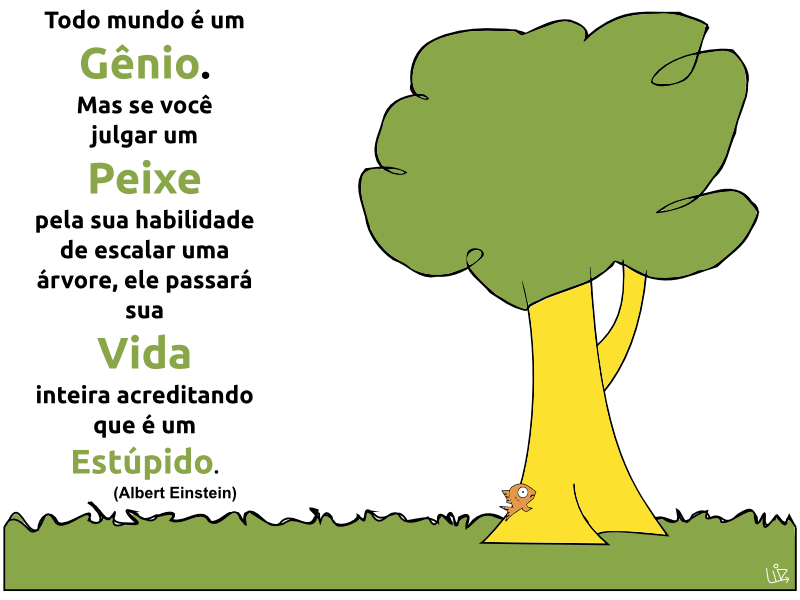
\includegraphics[scale=0.4]{figuras/todos-somos-genios}
 \caption{Exemplo de Figura.}
 \label{figurateste1}
\end{figure}

\begin{figure}[htb]
 \centering
  
\includegraphics[scale=0.8]{figuras/tux}
  \caption[Legenda mais curta.]{Esse é um exemplo de figura com legenda muito grande, que tem por objetivo mostrar como o espaço entre linhas será simples.}
  \label{figurateste2}
\end{figure}

\section{Segunda seção da Revisão.}

Em \eqref{equacao1} temos um exemplo de texto matemático com numeração\index{equação com numeração}. E logo depois 
temos um exemplo de texto matemático sem numeração.
%Note que o comando \index é usado para inserir "equação com numeração" no Índice.

\begin{equation}\label{equacao1}
 \int_a^b f'(x)\,dx = f(b) - f(a)
\end{equation}

\begin{equation}\nonumber
 \int_a^b f'(x)\,dx = f(b) - f(a)
\end{equation}

Aqui está mais outro exemplo de referência \cite{Autor4}.

\end{comment}
